\begin{figure*}
\begin{center}
    \captionsetup{type=figure}
    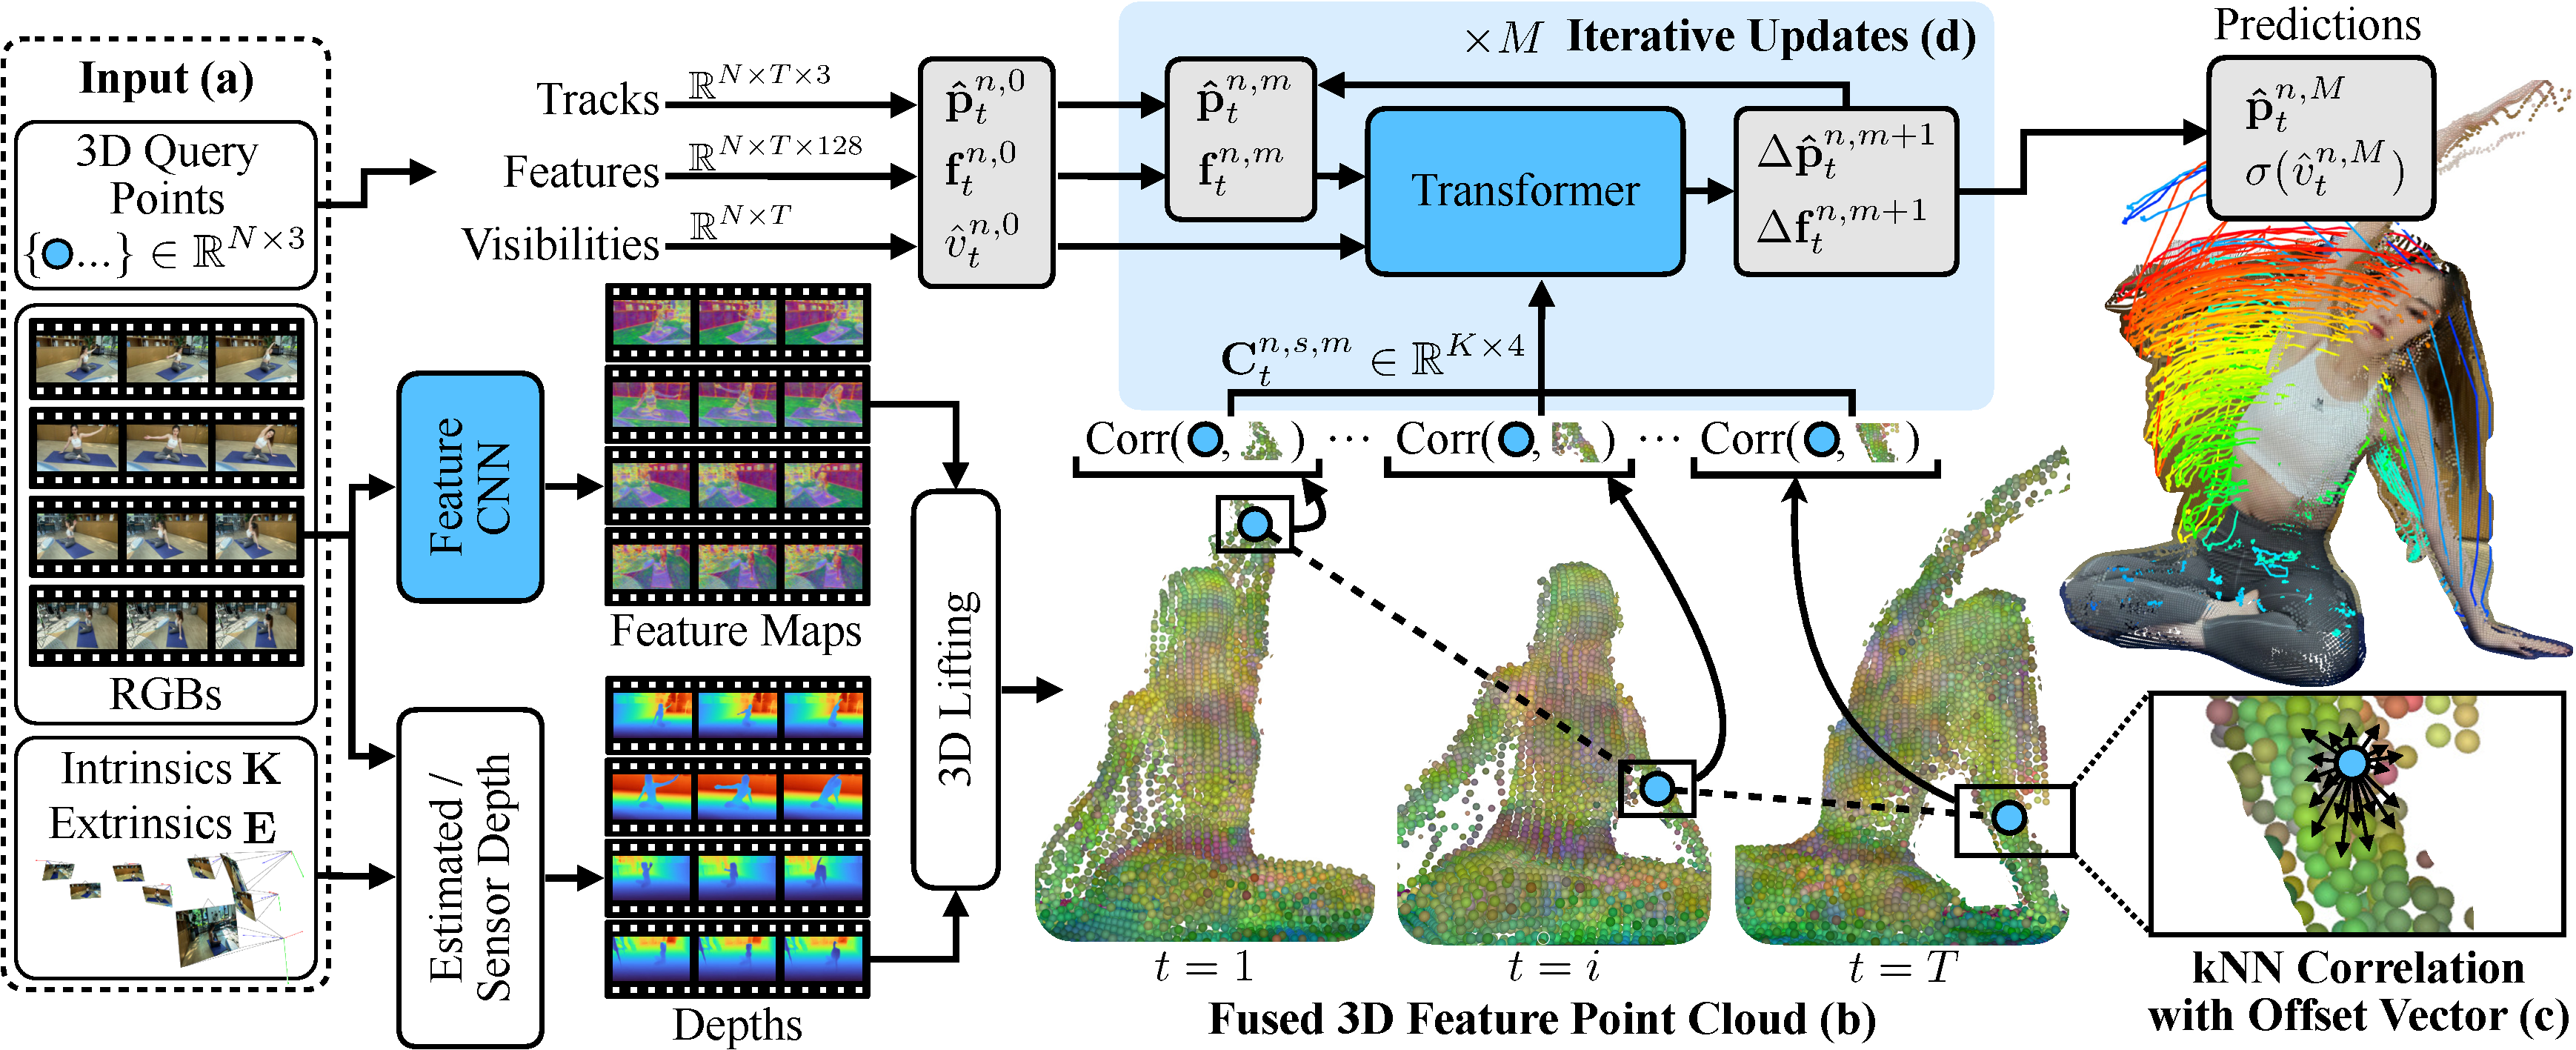
\includegraphics[width=\linewidth]{figures/pipeline_july_v3.optimized-prepress.pdf}
    \vspace{-0.27in}
    \captionof{figure}{
    \textbf{MVTracker Pipeline}. 
    (a) Given synchronized multi-view RGB videos with known intrinsics and extrinsics, we extract per-view feature maps using a CNN-based encoder. (b) We construct a point cloud from estimated or sensor-based depth maps, associating each point with learned feature embeddings (\cref{sec:fused-point-cloud}). (c) We compute directed kNN-based correlation within the point cloud, capturing spatiotemporal relationships across views (\cref{sec:multi-scale-spatial-correlation}). (d) A transformer-based update module iteratively refines point trajectories using self-attention over multi-view feature correlations within a sliding temporal window (\cref{sec:Transformer}). (e) The model processes sequences in overlapping sliding windows, producing temporally consistent 3D point trajectories with occlusion-aware visibility predictions (\cref{sec:windowed-inference-and-unrolled-training}). The blue blocks denote trainable neural models. The visualized sequence is from SelfCap~\cite{xu2024longvolcap_selfcap} and uses DUSt3R~\cite{wang2024dust3r} to estimate depth.
    }
    \label{fig:pipeline}
\end{center}
\end{figure*}
